\documentclass{article}
\usepackage[utf8]{inputenc}
\usepackage{listings}
\usepackage{xcolor}
\usepackage[justification=centering]{caption}
\usepackage{float}
\usepackage{amsmath}

% --- Colour definitions ---
\definecolor{codegreen}{rgb}{0,0.6,0}
\definecolor{codegray}{rgb}{0.5,0.5,0.5}
\definecolor{codepurple}{rgb}{0.58,0,0.82}
\definecolor{backcolour}{rgb}{0.95,0.95,0.92}

% --- PDDL/JSHOP2 language definition ---
\lstdefinelanguage{PDDL}{
  sensitive=false,
  morecomment=[l]{;},
  alsoletter={-,:},
  morekeywords={
    define, domain, problem, and, or, not, imply, exists, forall, when,
    increase, decrease, assign, scale-up, scale-down,
    :domain, :requirements, :types, :constants, :predicates, :functions,
    :action, :parameters, :precondition, :effect,
    :durative-action, :duration, :condition,
    :objects, :init, :goal, :metric,
    defdomain, defproblem, :operator, :method, :-
  }
}

\lstset{
  language=PDDL,
  backgroundcolor=\color{backcolour},
  commentstyle=\color{codegreen}\itshape,
  keywordstyle=\color{blue}\bfseries,
  numberstyle=\tiny\color{codegray},
  stringstyle=\color{codepurple},
  basicstyle=\ttfamily\footnotesize,
  breakatwhitespace=false,
  breaklines=true,
  captionpos=b,
  keepspaces=true,
  numbers=left,
  numbersep=5pt,
  showspaces=false,
  showstringspaces=false,
  showtabs=false,
  tabsize=2
}

\usepackage{graphicx}

\title{Hierarchical Planning with JSHOP2}
\author{Aleksandra S\l{}omska \\ Zofia Narloch}

\begin{document}

\maketitle

% ============================================================
\section{Exercise 1.1: Emergency Service Logistics, Initial Release}
% ============================================================

In this exercise we recreated the Emergency Service Logistics domain from the PDDL labs, but this time using JSHOP2, which is a hierarchical planner. The main difference is that instead of just describing what actions are possible (like in PDDL), we also have to tell the planner how to organise those actions into higher-level tasks.

Below is an example problem we defined for JSHOP2. There are three people, three locations and three crates:

\begin{lstlisting}
(defproblem problem p1
  (
    (drone-at drone1 depot)
    (crate-at crate1 depot)
    (crate-at crate2 depot)
    (crate-at crate3 depot)
    (empty-arm drone1 left)
    (empty-arm drone1 right)
    (content-crate food crate1)
    (content-crate food crate2)
    (content-crate medicine crate3)
    (person-at person1 loc1)
    (person-at person2 loc3)
    (person-at person3 loc2)
    (needs-content person2 food)
    (needs-content person2 medicine)
    (needs-content person3 food)
  )
  (
    (deliver-all)
  )
)
\end{lstlisting}

Here the goal is just \texttt{(deliver-all)} --- a single high-level task. In PDDL we would instead list each individual goal condition, like \texttt{(has-content-person person2 food)}. In JSHOP2 we let the task hierarchy figure out what needs to be done.

The planner produced the following plan:

\begin{lstlisting}[caption={First problem and the outcome - three people and three boxes}]
(!pick-up-crate crate1 depot drone1 left)
(!drone-move depot loc3 drone1)
(!drop-crate loc3 person2 crate1 left food drone1)
(!drone-move loc3 depot drone1)
(!pick-up-crate crate3 depot drone1 right)
(!drone-move depot loc3 drone1)
(!drop-crate loc3 person2 crate3 right medicine drone1)
(!drone-move loc3 depot drone1)
(!pick-up-crate crate2 depot drone1 left)
(!drone-move depot loc2 drone1)
(!drop-crate loc2 person3 crate2 left food drone1)
--------------------
Time Used = 0.009
\end{lstlisting}

The plan looks very similar to what PDDL planners produce --- the individual actions are the same. The difference is in how the planner found the plan.

\begin{figure}[H]
    \centering
    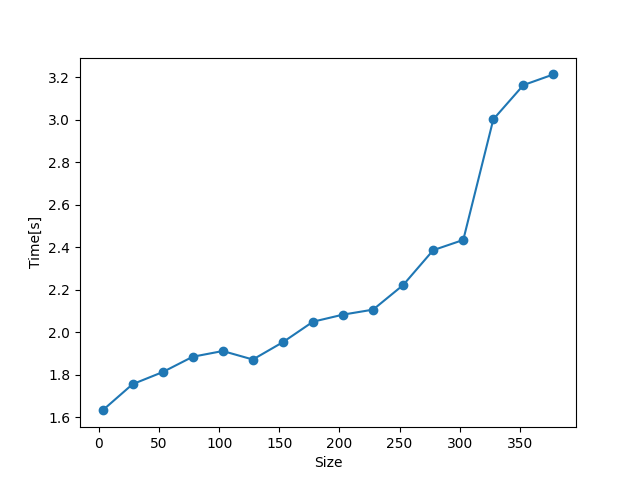
\includegraphics[width=0.9\textwidth]{Figure_1}
    \caption{Problem size vs.\ planning time for Exercise~1.1}
    \label{fig:figure1}
\end{figure}

It is important to note that the time shown on the graph is measured by the Python script. The time reported by JSHOP2 itself was below 1 second for every single problem. The graph shows that even at size 380 the total time was around 3.2 seconds --- and most of that is overhead from the Python script.

\subsection{Comparison with Classical Planning (BFS from Exercise 1.3)}

In Part 1.3 of the PDDL project, we tested several search algorithms. The best performing one was BFS (Breadth-First Search) with no heuristic. It solved a problem of size 17 in just 0.77 seconds. That was the largest problem any algorithm could solve within the 60-second time limit.

JSHOP2 solved a problem of size 380 in under one second of actual planning time. That is more than 22 times larger.

BFS works by expanding every possible state one step at a time, level by level. The number of states grows fast as the problem gets bigger: by size 17, BFS was already hitting the 60-second limit. JSHOP2 does not search through states in the same way --- it follows a task hierarchy defined in the domain file. The top-level task \texttt{(deliver-all)} is broken down into smaller tasks, which are broken down further into concrete actions.

The downside is that JSHOP2 does not guarantee an optimal plan. In the example above, the drone goes to \texttt{loc3} twice (for food and medicine separately for \texttt{person2}), even though it could carry both crates at once. BFS would find the shortest possible plan.

\subsection{Advantages of Hierarchical Planning}

\begin{itemize}
    \item \textbf{Scalability.} While BFS could not go past size 17, JSHOP2 handled size 380.
    \item \textbf{Speed.} The planner commits to a plan quickly by following the hierarchy; there is no exhaustive search.
\end{itemize}

\subsection{Disadvantages of Hierarchical Planning}

\begin{itemize}
    \item \textbf{No optimality guarantee.} JSHOP2 made two separate trips to deliver to \texttt{person2} even though one trip would have sufficed.
    \item \textbf{More work upfront.} Writing the JSHOP2 domain requires designing the full task hierarchy and defining methods for every situation.
\end{itemize}

% ============================================================
\section{Exercise 1.2: Advanced Emergency Logistics Domain}
% ============================================================

In the second part of the exercise we upgraded our JSHOP2 domain to handle more realistic logistics using numerical fluents and carrier. The domain moves away from individual named crates and instead tracks aggregate quantities of goods at locations, making the representation much more compact and scalable.

\subsection{Key Representational Changes}

Unlike Part~1, where every crate was a distinct object, the advanced domain represents supply as numeric quantities:

\begin{itemize}
    \item \texttt{(crates-at food depot 4)} -- 4 food boxes are at the depot.
    \item \texttt{(needs food loc3 1)} -- location \texttt{loc3} needs 1 food box.
    \item \texttt{(carrier-at carrier1 depot)} and \texttt{(carrier-capacity carrier1 5)} -- a carrier with capacity 5 is parked at the depot.
    \item \texttt{(carrier-content carrier1 food 0)} -- the carrier currently carries no food.
    \item \texttt{(reserved carrier1 food loc3 4)} -- 4 food boxes are reserved for \texttt{loc3} in \texttt{carrier1}.
\end{itemize}

This numeric representation removes the need to enumerate individual crate objects and allows the planner to reason about partial loads and bulk deliveries using calls such as \texttt{(call >= ?count 1)}.

\subsection{Delivery Strategy}

The \texttt{deliver-all} method selects among four branches, tried in order of priority:

\begin{enumerate}
    \item \textbf{Arm delivery for small needs (\texttt{use-drone-arms-small}).} When the greatest remaining need is at most~2 boxes, the drone uses its own arms (left/right) instead of a carrier. The \texttt{fill-arms} method loads one box per free arm, and \texttt{dispatch-arms} flies to each target location, drops the box, and returns to the depot.
    \item \textbf{Carrier fits the need (\texttt{use-carrier-fits}).} A carrier whose capacity $\geq$ the need is selected. Among all fitting carriers, the smallest one is chosen via the \texttt{better-fitting-carrier-exists} axiom.
    \item \textbf{No carrier fits (\texttt{use-carrier-partial}).} When no single carrier can hold the entire need, the largest available carrier is selected via the \texttt{larger-available-carrier-exists} axiom, and it is filled to capacity.
    \item \textbf{Arm fallback (\texttt{use-drone-arms}).} When no carrier is available at all (or none was selected by the above branches), the drone delivers one box per arm.
\end{enumerate}

For carrier-based branches, each dispatch cycle has two phases:

\begin{enumerate}
    \item \textbf{Filling phase.} The drone stays at the depot and loads boxes into the chosen carrier via the \texttt{fill-specific} and \texttt{fill-any} methods. Loading continues until the carrier is full or all current needs are reserved.
    \item \textbf{Dispatch phase.} The drone flies the carrier along a multi-stop route via the \texttt{dispatch-carrier} method, calling \texttt{!unload-carrier} at each reserved location before returning to the depot.
\end{enumerate}

After each return to depot, \texttt{deliver-all} recurses and re-evaluates the remaining needs, selecting the next best branch.

\subsection{Carrier Selection with Axioms}

Carrier selection is driven by axioms that evaluate the current state at planning time:

\begin{itemize}
    \item \textbf{\texttt{better-fitting-carrier-exists ?need ?cap}} --- true if a carrier with capacity $\geq$ \texttt{need} but $<$ \texttt{cap} exists. Used to ensure the smallest fitting carrier is always chosen first.
    \item \textbf{\texttt{carrier-can-fit ?need}} --- true if at least one carrier can fit the entire need in one load.
    \item \textbf{\texttt{larger-available-carrier-exists ?cap}} --- true if a larger carrier than the current candidate exists. Used when no carrier fits the need, to ensure the largest available is chosen.
    \item \textbf{\texttt{greater-need-exists ?count}} --- true if any location has a higher need than the current one being considered. This implements a greater priority.
\end{itemize}

The \texttt{deliver-all} method tries four branches in order:

\begin{lstlisting}[caption={Delivery branches in deliver-all (p3\_3)}]
use-drone-arms-small
(
  (needs ?type ?loc ?need-count)
  (call <= ?need-count 2)
  (call >= ?need-count 1)
  (not (greater-need-exists ?need-count))
  (empty-arm drone1 ?arm)
)

use-carrier-fits
(
  (needs ?type ?loc ?need-count) 
  (call >= ?need-count 1)
  (not (greater-need-exists ?need-count))
  (carrier-at ?carrier depot)
  (carrier-capacity ?carrier ?cap)
  (call >= ?cap ?need-count)
  (not (better-fitting-carrier-exists ?need-count ?cap))
)

use-carrier-partial
(
  (needs ?type ?loc ?need-count) 
  (call >= ?need-count 1)
  (not (greater-need-exists ?need-count))
  (not (carrier-can-fit ?need-count))
  (carrier-at ?carrier depot)
  (carrier-capacity ?carrier ?cap)
  (not (larger-available-carrier-exists ?cap))
)

use-drone-arms
(
  (needs ?type ?loc ?need-count)
  (call >= ?need-count 1)
  (empty-arm drone1 ?arm)
)
\end{lstlisting}

\subsection{Partial and Full Loading}

The \texttt{fill-any} and \texttt{fill-specific} method handles two sub-cases:

\begin{itemize}
    \item \textbf{\texttt{load-fits}} -- the entire remaining need fits in the available capacity; all of it is reserved and loaded.
    \item \textbf{\texttt{load-partial}} -- the need exceeds the remaining capacity; only some boxes are reserved and loaded, leaving the rest for a future cycle.
\end{itemize}

\subsection{Arm-Based Delivery: fill-arms and dispatch-arms}

Both the \texttt{use-drone-arms-small} and the fallback \texttt{use-drone-arms} branches use the same sub-methods:

\begin{itemize}
    \item \textbf{\texttt{fill-arms}} recursively loads one box per free arm using the \texttt{!pick-up-crate-arm} operator. This operator simultaneously picks up a box from the depot and reserves the destination by decrementing the \texttt{needs} counter. Loading stops when either no empty arms remain or all needs are satisfied.
    \item \textbf{\texttt{dispatch-arms}} recursively visits each target location, drops the held box with \texttt{!drop-crate-arm}, and continues until the drone's arms are empty. It then returns the drone to the depot.
\end{itemize}

\begin{lstlisting}[caption={Arm-based delivery flow in deliver-all}]
use-drone-arms-small  
(
  ...
)
(
  (move-drone-alone drone1 depot)
  (fill-arms drone1)       
  (dispatch-arms drone1)   
  (deliver-all)            
)
\end{lstlisting}

The \texttt{use-drone-arms-small} branch is an optimisation: when the greatest remaining need is small ($\leq 2$), the drone's arms are sufficient, and deploying a carrier would be higher cost. The fallback \texttt{use-drone-arms} branch handles any remaining needs when no carriers are available.

\subsection{Flight Cost Model}

The cost of moving a drone without a carrier has a fixed cost of 50. Moving a carrier adds an additional cost proportional to its capacity, that is why a heavier or larger vehicle is more expensive to operate:

\[
  \text{cost}(\text{carrier move}) = 50 + \frac{\text{capacity}}{10}
\]

For example, a carrier with capacity 100 costs 60 per flight, while a capacity-5 carrier costs 50.5. This makes the planner to use smaller carrier when they are sufficient.

\subsection{Handling the Required Situations}

Table~\ref{tab:situations} summarises how each of the 11 required situations is handled by the domain.

\begin{table}[H]
\centering
\footnotesize
\begin{tabular}{|c|p{7.5cm}|p{4.5cm}|}
\hline
\textbf{\#} & \textbf{Situation} & \textbf{Mechanism} \\ \hline
1 & No carrier available & \texttt{use-drone-arms} \\ \hline
2 & One carrier available & \texttt{use-carrier-fits}, \texttt{use-carrier-partial} \\ \hline
3 & Different box types on the same carrier & \texttt{fill-specific}, \texttt{fill-any} \\ \hline
4 & Remaining boxes delivered without carrier after carrier cycle & \texttt{deliver-all} $\to$ \texttt{use-drone-arms} \\ \hline
5 & carrier smaller than need $\to$ load to max capacity & \texttt{load-partial} in \texttt{fill-specific}/\texttt{fill-any} \\ \hline
6 & carrier larger than need $\to$ load only what is needed & \texttt{load-fits} in \texttt{fill-specific}/\texttt{fill-any} \\ \hline
7 & Multiple carriers fit $\to$ choose smallest fitting & \texttt{better-fitting-carrier-exists} axiom \\ \hline
8 & No carrier fits $\to$ choose largest available & \texttt{larger-available-carrier-exists} axiom \\ \hline
9 & Re-evaluate after each depot return & \texttt{deliver-all}, \texttt{dispatch-carrier} \\ \hline
10 & Serve location with greatest need first & \texttt{greater-need-exists} \\ \hline
11 & Multi-location trip without returning to depot & \texttt{dispatch-carrier} \\ \hline
\end{tabular}
\caption{The 11 required situations and how they are handled in the domain.}
\label{tab:situations}
\end{table}

\subsection{Scalability Comparison}

The P2 domain produces plans much faster than the P1 domain for problems with many deliveries, because needs are acumulated per location. Instead of making one trip per crate, the planner loads an entire carrier and serves multiple locations in one dispatch cycle, reducing the total number of operators in the plan and the depth of the search.

\end{document}